\documentclass[12pt,parskip=full]{scrartcl}

\usepackage{../00-common/uebungsblatt}

\begin{document}

\xheader{1}{Arbeiten mit Python und Jupyter Notebooks}

Erstellen Sie das Jupyter Notebook \uebdatei{} und lösen Sie darin die folgenden Aufgaben.

\aufgabe{Erzeugen Sie die Matrix}
  \begin{displaymath}
    \mathbf{A}
    =
    \begin{pmatrix}
     1 &     2 &     3 &     4 &     5 &     6 &     7 &     8 &     9 &    10 \\
     2 &     3 &     4 &     5 &     6 &     7 &     8 &     9 &    10 &    11 \\
     3 &     4 &     5 &     6 &     7 &     8 &     9 &    10 &    11 &    12 \\
     4 &     5 &     6 &     7 &     8 &     9 &    10 &    11 &    12 &    13 \\
     5 &     6 &     7 &     8 &     9 &    10 &    11 &    12 &    13 &    14 \\
     6 &     7 &     8 &     9 &    10 &    11 &    12 &    13 &    14 &    15 \\
     7 &     8 &     9 &    10 &    11 &    12 &    13 &    14 &    15 &    16 \\
     8 &     9 &    10 &    11 &    12 &    13 &    14 &    15 &    16 &    17 \\
     9 &    10 &    11 &    12 &    13 &    14 &    15 &    16 &    17 &    18 \\
    10 &    11 &    12 &    13 &    14 &    15 &    16 &    17 &    18 &    19 \\
    \end{pmatrix}
  \end{displaymath}  
  ohne die Werte einzeln einzugeben. Verwenden Sie eine Schleife und die NumPy-Funktion \mc{np.arange}.

\aufgabe{Plotten}


\teilaufgabe{Plotten Sie die Funktionen}
  % y1 = sin(3 * pi * sin(x))
  % y2 = cos(exp(0.7 * x))
  \begin{displaymath}
    f(x) = \sin(3 \pi \sin x)
    \quad \text{und} \quad
    g(x) = \cos(e^{0.7 x})
  \end{displaymath}
  für $0 \leq x \leq 2 \pi$ jeweils in einem eigenen Koordinatensystem. Wie viele Punkte auf der $x$-Achse werden jeweils benötigt, um eine gute Darstellung der Funktionen zu erreichen?

\clearpage

\teilaufgabe{Ein Spirograph ist ein Spielzeug mit dem so genannte Roulette-Kurven erzeugt werden können. 
 \begin{center}
    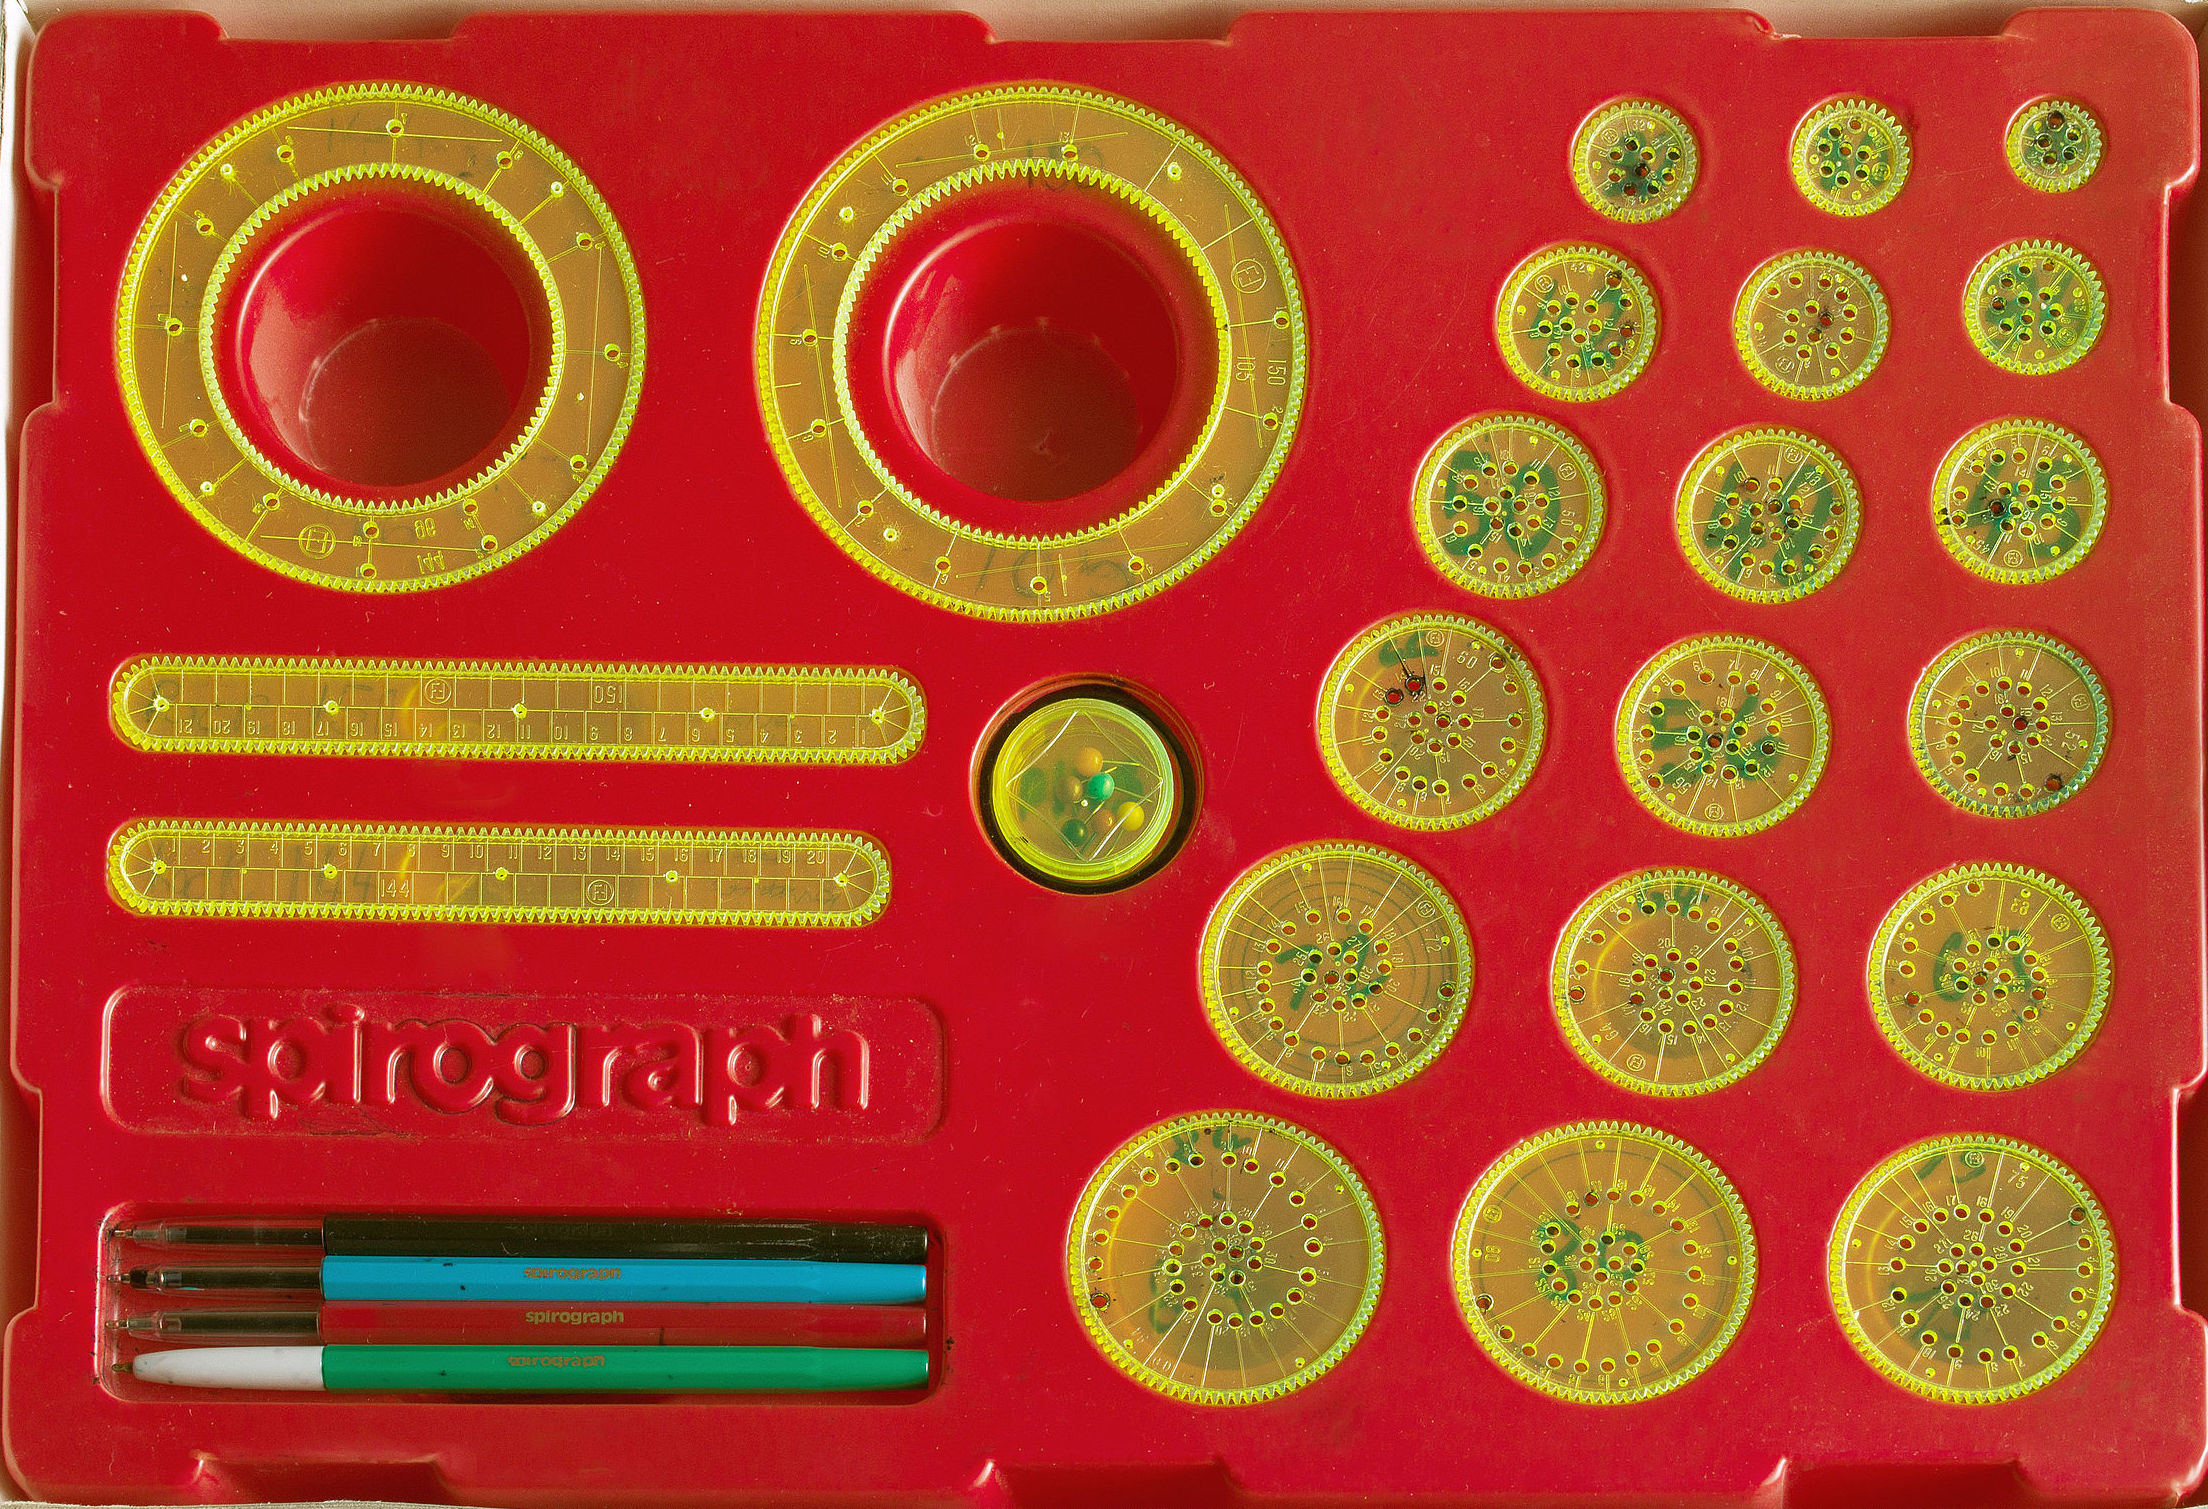
\includegraphics[height=34mm]{Spirograph_set_(UK_Palitoy_early_1980s)_(perspective_fixed)}
    \hspace*{10mm}
    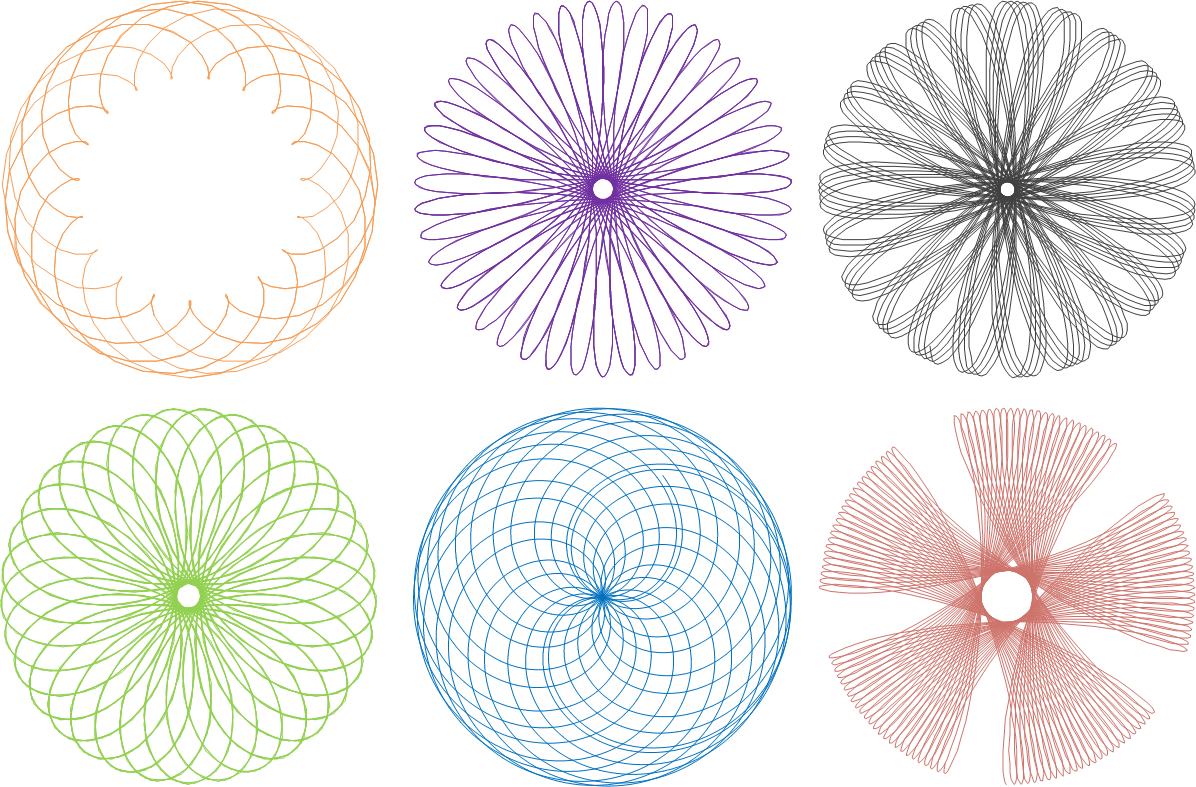
\includegraphics[height=34mm]{SPIROGRAPH}      
\end{center}
 Mathematisch werden diese durch die parametrische Kurve
  \begin{displaymath}
    \mathbf{y}(t) = 
    \begin{pmatrix}
      (1-k) \cos(t) + l k \cos \left(\frac{1-k}{k}t\right),\\[4pt]
      (1-k) \sin(t) - l k \sin \left(\frac{1-k}{k}t\right)
    \end{pmatrix}
  \end{displaymath}
  beschrieben. Plotten Sie für $k = 0.82$ und $l = 0.35$ den Verlauf der Kurve für $0 \leq t \leq 100 \pi$. Experimentieren Sie mit den Parametern $l$ und $k$!
}

\aufgabe{Eigene Funktionen erstellen}

\teilaufgabe{Erstellen Sie eine Python-Funktion \mc{pwfunc} (piecewise-function) zu dem  dargestellten Graphen. Plotten Sie die Funktion zur Kontrolle mit \mc{plot}. 
  
  \begin{center}
    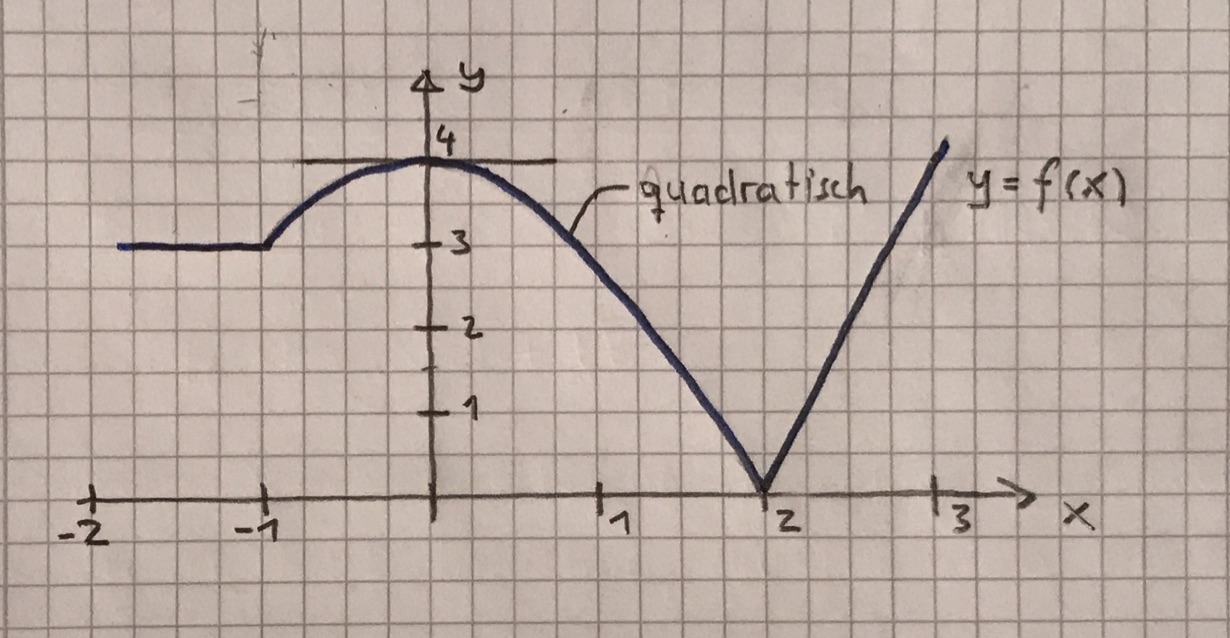
\includegraphics[width=80mm]{pwfunc}
  \end{center}
}

\teilaufgabe{Wir betrachten die Funktionenschar $f_a : \R \to \R$ mit $f_a(x) = e^{ax}$. Erstellen Sie eine Python-Funktion, die für einen Wert $a$ die Funktion $f_a$ zurückliefert. Plotten Sie $f_a$ für $a = -2, -1.8, \dots, 1.8, 2$ und $x \in [-2, 2]$.
}

\end{document}
